% ================================================================
% The printable version of latex/starters/targeted/KS4/geometry/trigBearingsStarter01.tex
%
% This is the same deck, laid out to be handed out rather than put on
% the board. Every slide is shown as it stands before any answer is
% revealed, and 4 copies of it go on one page of A4, two by two, so
% that a printed page cuts into four question sheets.
%
%   made from           latex/starters/targeted/KS4/geometry/trigBearingsStarter01.tex
%   slides on the sheet 1
%   copies of each      4, two by two on A4 landscape
%   printing rules      version 1
%
% Nothing was reworded and nothing was rewritten. Each slide is the slide
% from the deck, asked for at its first step, which is how the answers
% stay hidden.
%
% Please don't edit this file. It is written again from the one it was
% made from whenever that changes, so an edit here would be lost - edit
% that file instead and this one follows.
% ================================================================
\documentclass[aspectratio=169]{beamer}
\usepackage{amsmath}
\usepackage{tikz}
\usetikzlibrary{angles,quotes,calc}

% ================================================================
% Answer-overlay helpers
% ================================================================
\newcommand{\ablank}[1]{%
  \alt<2>{\textcolor{red}{#1}}{\underline{\phantom{#1}}}%
}
\newcommand{\ashow}[1]{\uncover<2->{\textcolor{red}{\small #1}}}
\newcommand{\ashowq}[1]{\alt<2->{\textcolor{red}{\small #1}}{?}}

% Answers drawn straight on to a TikZ diagram, revealed on overlay 2 like \ashow.
% Space is reserved on overlay 1, so the diagram does not move between slides.
\usetikzlibrary{overlay-beamer-styles}
\tikzset{
  ans/.style     = {red, thick, visible on=<2->},
  ansfill/.style = {red!15, visible on=<2->},
  anslab/.style  = {red, font=\tiny, visible on=<2->},
}

\title{Starter}
\author{}
\date{}

\setbeamertemplate{navigation symbols}{}

% ---------------------------------------------------------------
% Added so this deck prints four slides to a page. Nothing above
% this line was changed.
% ---------------------------------------------------------------
\usepackage{pgfpages}

% 4 slides to a sheet of A4, two by two, with a thin line round each
% so that the page can be cut up. The margin is wide enough that the lines
% fall inside what a printer can actually put ink on.
\pgfpagesuselayout{4 on 1}[a4paper,landscape,border shrink=10mm]
\pgfpageslogicalpageoptions{1}{border code=\pgfusepath{stroke}}
\pgfpageslogicalpageoptions{2}{border code=\pgfusepath{stroke}}
\pgfpageslogicalpageoptions{3}{border code=\pgfusepath{stroke}}
\pgfpageslogicalpageoptions{4}{border code=\pgfusepath{stroke}}

% There is nothing on paper to click, and a slide announcing a new section
% would sit between two copies of the same question and put every page after
% it out of step with the grid.
\setbeamertemplate{navigation symbols}{}
\AtBeginPart{}
\AtBeginSection{}
\AtBeginSubsection{}
\AtBeginSubsubsection{}
\begin{document}

\begin{frame}<1>
  \frametitle{Starter}

  \begin{columns}[t,onlytextwidth]

    % ===== LEFT COLUMN =====
    \begin{column}{0.4\textwidth}
      % ------------------ Q1 ------------------
      \textbf{1.}


      \vspace{0.7em}
      Which pairs of cardinal directions (North, South, East, West) meet at right angles?

      \ashow{North and East, North and West, South and East, South and West.}

      % ----- Flexible space -----
      \vfill
      \vspace{3em}

      % ------------------ Q3 ------------------
      \textbf{3.}

      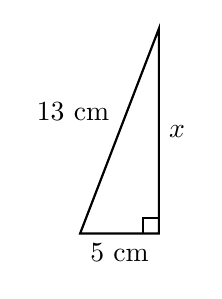
\begin{tikzpicture}[scale=0.2, thick]
        % Right triangle (hypotenuse is 13)
        \coordinate (A) at (0,0);
        \coordinate (B) at (5,0);
        \coordinate (C) at (5,13);

        % Triangle
        \draw (A) -- (B) -- (C) -- cycle;

        % Right angle marker
        \draw ($(B)+(0,1)$) -- ($(B)+(-1,1)$) -- ($(B)+(-1,0)$);

        % Side lengths
        \node[below] at ($(A)!0.5!(B)$) {$5$ cm};
        \node[right] at ($(B)!0.5!(C)$) {$x$};
        \node[above left] at ($(A)!0.5!(C)$) {$13$ cm};

      \end{tikzpicture}

      \vspace{0.5em}
      Find the missing side.

      \ashow{$x = 12$ cm}

    \end{column}

    % ===== RIGHT COLUMN =====
    \begin{column}{0.6\textwidth}
      % ------------------ Q2 ------------------
      
      \textbf{2.}

      \begin{columns}[t,onlytextwidth]
      \begin{column}{0.5\textwidth}

      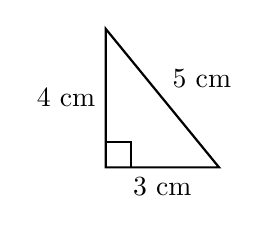
\begin{tikzpicture}[scale=0.8, thick]

        % Coordinates of triangle (hypotenuse longest)
        \coordinate (A) at (0,0);
        \coordinate (B) at (1.8,0);
        \coordinate (C) at (0,2.2);

        % Draw triangle
        \draw (A) -- (B) -- (C) -- cycle;

        % Right angle marker
        \draw ($(A)+(0,0.4)$) -- ($(A)+(0.4,0.4)$) -- ($(A)+(0.4,0)$);

        % Label sides
        \node[below] at ($(A)!0.5!(B)$) {3 cm};
        \node[left]  at ($(A)!0.5!(C)$) {4 cm};
        \node[above right] at ($(B)!0.5!(C)$) {5 cm};

      \end{tikzpicture}
\end{column}
      \begin{column}{0.5\textwidth}
      Which side is the hypotenuse?

      \ashow{The side labelled 5 cm is the hypotenuse.}
\end{column}

    \end{columns}

\textbf{4.}

\begin{columns}[t,onlytextwidth]
  % ===== Diagram Column =====
  \begin{column}{0.45\textwidth}

    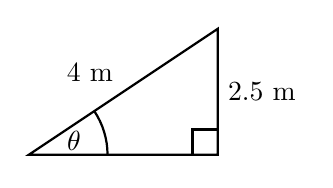
\begin{tikzpicture}[scale=0.8, thick]
      % Triangle for inverse sine
      \coordinate (A) at (0,0);
      \coordinate (B) at (3,0);
      \coordinate (C) at (3,2);

      % Draw triangle
      \draw (A) -- (B) -- (C) -- cycle;

      % Right angle
      \draw ($(B)+(0,0.4)$) -- ($(B)+(-0.4,0.4)$) -- ($(B)+(-0.4,0)$);

      % Side labels
      \node[right] at ($(B)!0.5!(C)$) {$2.5$ m};  % opposite
      \node[above left] at ($(A)!0.5!(C)$) {$4$ m}; % hypotenuse

      % Angle θ at A
      \pic[draw,angle radius=10mm,"$\theta$"{scale=1}] {angle = B--A--C};

    \end{tikzpicture}

  \end{column}

  % ===== Options Column =====
  \begin{column}{0.55\textwidth}

    Find $\theta$.

     \fontsize{10}{12}\selectfont

    \begin{itemize}
        \item[(A)] $\displaystyle \theta = \sin^{-1}\!\left(\frac{2.5}{4}\right)$
        \item[(B)] $\displaystyle \theta = \cos^{-1}\!\left(\frac{2.5}{4}\right)$
        \item[(C)] $\displaystyle \theta = \tan^{-1}\!\left(\frac{2.5}{4}\right)$
    \end{itemize}

    \ashow{Answer: (A)}

  \end{column}
\end{columns}
\end{column}
\end{columns}

\end{frame}
\begin{frame}<1>
  \frametitle{Starter}

  \begin{columns}[t,onlytextwidth]

    % ===== LEFT COLUMN =====
    \begin{column}{0.4\textwidth}
      % ------------------ Q1 ------------------
      \textbf{1.}


      \vspace{0.7em}
      Which pairs of cardinal directions (North, South, East, West) meet at right angles?

      \ashow{North and East, North and West, South and East, South and West.}

      % ----- Flexible space -----
      \vfill
      \vspace{3em}

      % ------------------ Q3 ------------------
      \textbf{3.}

      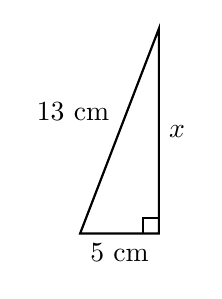
\begin{tikzpicture}[scale=0.2, thick]
        % Right triangle (hypotenuse is 13)
        \coordinate (A) at (0,0);
        \coordinate (B) at (5,0);
        \coordinate (C) at (5,13);

        % Triangle
        \draw (A) -- (B) -- (C) -- cycle;

        % Right angle marker
        \draw ($(B)+(0,1)$) -- ($(B)+(-1,1)$) -- ($(B)+(-1,0)$);

        % Side lengths
        \node[below] at ($(A)!0.5!(B)$) {$5$ cm};
        \node[right] at ($(B)!0.5!(C)$) {$x$};
        \node[above left] at ($(A)!0.5!(C)$) {$13$ cm};

      \end{tikzpicture}

      \vspace{0.5em}
      Find the missing side.

      \ashow{$x = 12$ cm}

    \end{column}

    % ===== RIGHT COLUMN =====
    \begin{column}{0.6\textwidth}
      % ------------------ Q2 ------------------
      
      \textbf{2.}

      \begin{columns}[t,onlytextwidth]
      \begin{column}{0.5\textwidth}

      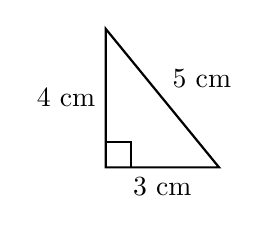
\begin{tikzpicture}[scale=0.8, thick]

        % Coordinates of triangle (hypotenuse longest)
        \coordinate (A) at (0,0);
        \coordinate (B) at (1.8,0);
        \coordinate (C) at (0,2.2);

        % Draw triangle
        \draw (A) -- (B) -- (C) -- cycle;

        % Right angle marker
        \draw ($(A)+(0,0.4)$) -- ($(A)+(0.4,0.4)$) -- ($(A)+(0.4,0)$);

        % Label sides
        \node[below] at ($(A)!0.5!(B)$) {3 cm};
        \node[left]  at ($(A)!0.5!(C)$) {4 cm};
        \node[above right] at ($(B)!0.5!(C)$) {5 cm};

      \end{tikzpicture}
\end{column}
      \begin{column}{0.5\textwidth}
      Which side is the hypotenuse?

      \ashow{The side labelled 5 cm is the hypotenuse.}
\end{column}

    \end{columns}

\textbf{4.}

\begin{columns}[t,onlytextwidth]
  % ===== Diagram Column =====
  \begin{column}{0.45\textwidth}

    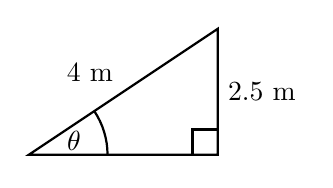
\begin{tikzpicture}[scale=0.8, thick]
      % Triangle for inverse sine
      \coordinate (A) at (0,0);
      \coordinate (B) at (3,0);
      \coordinate (C) at (3,2);

      % Draw triangle
      \draw (A) -- (B) -- (C) -- cycle;

      % Right angle
      \draw ($(B)+(0,0.4)$) -- ($(B)+(-0.4,0.4)$) -- ($(B)+(-0.4,0)$);

      % Side labels
      \node[right] at ($(B)!0.5!(C)$) {$2.5$ m};  % opposite
      \node[above left] at ($(A)!0.5!(C)$) {$4$ m}; % hypotenuse

      % Angle θ at A
      \pic[draw,angle radius=10mm,"$\theta$"{scale=1}] {angle = B--A--C};

    \end{tikzpicture}

  \end{column}

  % ===== Options Column =====
  \begin{column}{0.55\textwidth}

    Find $\theta$.

     \fontsize{10}{12}\selectfont

    \begin{itemize}
        \item[(A)] $\displaystyle \theta = \sin^{-1}\!\left(\frac{2.5}{4}\right)$
        \item[(B)] $\displaystyle \theta = \cos^{-1}\!\left(\frac{2.5}{4}\right)$
        \item[(C)] $\displaystyle \theta = \tan^{-1}\!\left(\frac{2.5}{4}\right)$
    \end{itemize}

    \ashow{Answer: (A)}

  \end{column}
\end{columns}
\end{column}
\end{columns}

\end{frame}
\begin{frame}<1>
  \frametitle{Starter}

  \begin{columns}[t,onlytextwidth]

    % ===== LEFT COLUMN =====
    \begin{column}{0.4\textwidth}
      % ------------------ Q1 ------------------
      \textbf{1.}


      \vspace{0.7em}
      Which pairs of cardinal directions (North, South, East, West) meet at right angles?

      \ashow{North and East, North and West, South and East, South and West.}

      % ----- Flexible space -----
      \vfill
      \vspace{3em}

      % ------------------ Q3 ------------------
      \textbf{3.}

      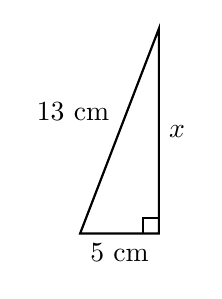
\begin{tikzpicture}[scale=0.2, thick]
        % Right triangle (hypotenuse is 13)
        \coordinate (A) at (0,0);
        \coordinate (B) at (5,0);
        \coordinate (C) at (5,13);

        % Triangle
        \draw (A) -- (B) -- (C) -- cycle;

        % Right angle marker
        \draw ($(B)+(0,1)$) -- ($(B)+(-1,1)$) -- ($(B)+(-1,0)$);

        % Side lengths
        \node[below] at ($(A)!0.5!(B)$) {$5$ cm};
        \node[right] at ($(B)!0.5!(C)$) {$x$};
        \node[above left] at ($(A)!0.5!(C)$) {$13$ cm};

      \end{tikzpicture}

      \vspace{0.5em}
      Find the missing side.

      \ashow{$x = 12$ cm}

    \end{column}

    % ===== RIGHT COLUMN =====
    \begin{column}{0.6\textwidth}
      % ------------------ Q2 ------------------
      
      \textbf{2.}

      \begin{columns}[t,onlytextwidth]
      \begin{column}{0.5\textwidth}

      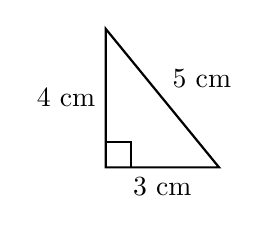
\begin{tikzpicture}[scale=0.8, thick]

        % Coordinates of triangle (hypotenuse longest)
        \coordinate (A) at (0,0);
        \coordinate (B) at (1.8,0);
        \coordinate (C) at (0,2.2);

        % Draw triangle
        \draw (A) -- (B) -- (C) -- cycle;

        % Right angle marker
        \draw ($(A)+(0,0.4)$) -- ($(A)+(0.4,0.4)$) -- ($(A)+(0.4,0)$);

        % Label sides
        \node[below] at ($(A)!0.5!(B)$) {3 cm};
        \node[left]  at ($(A)!0.5!(C)$) {4 cm};
        \node[above right] at ($(B)!0.5!(C)$) {5 cm};

      \end{tikzpicture}
\end{column}
      \begin{column}{0.5\textwidth}
      Which side is the hypotenuse?

      \ashow{The side labelled 5 cm is the hypotenuse.}
\end{column}

    \end{columns}

\textbf{4.}

\begin{columns}[t,onlytextwidth]
  % ===== Diagram Column =====
  \begin{column}{0.45\textwidth}

    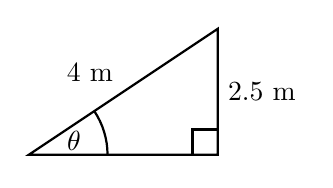
\begin{tikzpicture}[scale=0.8, thick]
      % Triangle for inverse sine
      \coordinate (A) at (0,0);
      \coordinate (B) at (3,0);
      \coordinate (C) at (3,2);

      % Draw triangle
      \draw (A) -- (B) -- (C) -- cycle;

      % Right angle
      \draw ($(B)+(0,0.4)$) -- ($(B)+(-0.4,0.4)$) -- ($(B)+(-0.4,0)$);

      % Side labels
      \node[right] at ($(B)!0.5!(C)$) {$2.5$ m};  % opposite
      \node[above left] at ($(A)!0.5!(C)$) {$4$ m}; % hypotenuse

      % Angle θ at A
      \pic[draw,angle radius=10mm,"$\theta$"{scale=1}] {angle = B--A--C};

    \end{tikzpicture}

  \end{column}

  % ===== Options Column =====
  \begin{column}{0.55\textwidth}

    Find $\theta$.

     \fontsize{10}{12}\selectfont

    \begin{itemize}
        \item[(A)] $\displaystyle \theta = \sin^{-1}\!\left(\frac{2.5}{4}\right)$
        \item[(B)] $\displaystyle \theta = \cos^{-1}\!\left(\frac{2.5}{4}\right)$
        \item[(C)] $\displaystyle \theta = \tan^{-1}\!\left(\frac{2.5}{4}\right)$
    \end{itemize}

    \ashow{Answer: (A)}

  \end{column}
\end{columns}
\end{column}
\end{columns}

\end{frame}
\begin{frame}<1>
  \frametitle{Starter}

  \begin{columns}[t,onlytextwidth]

    % ===== LEFT COLUMN =====
    \begin{column}{0.4\textwidth}
      % ------------------ Q1 ------------------
      \textbf{1.}


      \vspace{0.7em}
      Which pairs of cardinal directions (North, South, East, West) meet at right angles?

      \ashow{North and East, North and West, South and East, South and West.}

      % ----- Flexible space -----
      \vfill
      \vspace{3em}

      % ------------------ Q3 ------------------
      \textbf{3.}

      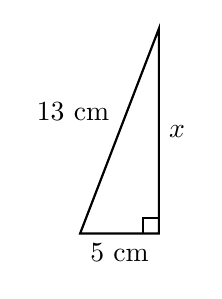
\begin{tikzpicture}[scale=0.2, thick]
        % Right triangle (hypotenuse is 13)
        \coordinate (A) at (0,0);
        \coordinate (B) at (5,0);
        \coordinate (C) at (5,13);

        % Triangle
        \draw (A) -- (B) -- (C) -- cycle;

        % Right angle marker
        \draw ($(B)+(0,1)$) -- ($(B)+(-1,1)$) -- ($(B)+(-1,0)$);

        % Side lengths
        \node[below] at ($(A)!0.5!(B)$) {$5$ cm};
        \node[right] at ($(B)!0.5!(C)$) {$x$};
        \node[above left] at ($(A)!0.5!(C)$) {$13$ cm};

      \end{tikzpicture}

      \vspace{0.5em}
      Find the missing side.

      \ashow{$x = 12$ cm}

    \end{column}

    % ===== RIGHT COLUMN =====
    \begin{column}{0.6\textwidth}
      % ------------------ Q2 ------------------
      
      \textbf{2.}

      \begin{columns}[t,onlytextwidth]
      \begin{column}{0.5\textwidth}

      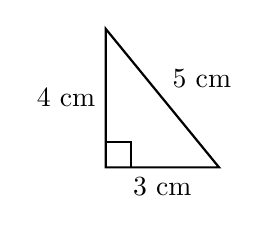
\begin{tikzpicture}[scale=0.8, thick]

        % Coordinates of triangle (hypotenuse longest)
        \coordinate (A) at (0,0);
        \coordinate (B) at (1.8,0);
        \coordinate (C) at (0,2.2);

        % Draw triangle
        \draw (A) -- (B) -- (C) -- cycle;

        % Right angle marker
        \draw ($(A)+(0,0.4)$) -- ($(A)+(0.4,0.4)$) -- ($(A)+(0.4,0)$);

        % Label sides
        \node[below] at ($(A)!0.5!(B)$) {3 cm};
        \node[left]  at ($(A)!0.5!(C)$) {4 cm};
        \node[above right] at ($(B)!0.5!(C)$) {5 cm};

      \end{tikzpicture}
\end{column}
      \begin{column}{0.5\textwidth}
      Which side is the hypotenuse?

      \ashow{The side labelled 5 cm is the hypotenuse.}
\end{column}

    \end{columns}

\textbf{4.}

\begin{columns}[t,onlytextwidth]
  % ===== Diagram Column =====
  \begin{column}{0.45\textwidth}

    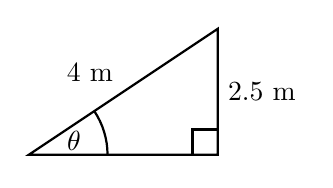
\begin{tikzpicture}[scale=0.8, thick]
      % Triangle for inverse sine
      \coordinate (A) at (0,0);
      \coordinate (B) at (3,0);
      \coordinate (C) at (3,2);

      % Draw triangle
      \draw (A) -- (B) -- (C) -- cycle;

      % Right angle
      \draw ($(B)+(0,0.4)$) -- ($(B)+(-0.4,0.4)$) -- ($(B)+(-0.4,0)$);

      % Side labels
      \node[right] at ($(B)!0.5!(C)$) {$2.5$ m};  % opposite
      \node[above left] at ($(A)!0.5!(C)$) {$4$ m}; % hypotenuse

      % Angle θ at A
      \pic[draw,angle radius=10mm,"$\theta$"{scale=1}] {angle = B--A--C};

    \end{tikzpicture}

  \end{column}

  % ===== Options Column =====
  \begin{column}{0.55\textwidth}

    Find $\theta$.

     \fontsize{10}{12}\selectfont

    \begin{itemize}
        \item[(A)] $\displaystyle \theta = \sin^{-1}\!\left(\frac{2.5}{4}\right)$
        \item[(B)] $\displaystyle \theta = \cos^{-1}\!\left(\frac{2.5}{4}\right)$
        \item[(C)] $\displaystyle \theta = \tan^{-1}\!\left(\frac{2.5}{4}\right)$
    \end{itemize}

    \ashow{Answer: (A)}

  \end{column}
\end{columns}
\end{column}
\end{columns}

\end{frame}

\end{document}